\section{\label{sec:level1}Experimental Results}
\subsection{Quantum Process Tomography}

\begin{figure}[b]
\centering
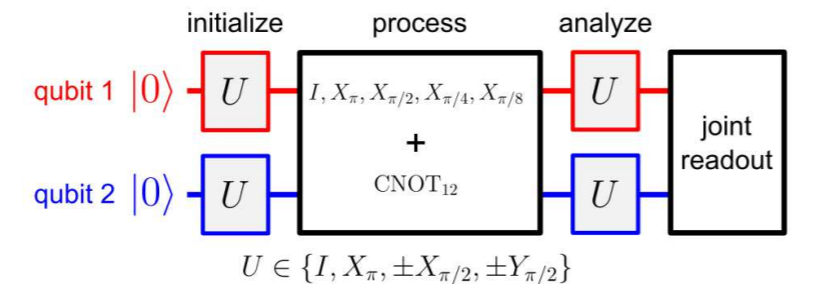
\includegraphics[height=0.19\textwidth,keepaspectratio]{ptcircuit}
\caption{\label{fig:ptcircuit}Gate sequence to perform QPT. The unitary operators, $U$ are used to prepare various input states and the pulses after the process enable state tomography analysis $^{[}$\citep{Chow2012UniversalQubits}$^{]}$.}
\end{figure}


The tunability of a selection of the 19Q processor enables, in addition to single qubit gates, two-qubit gates to be completed. To complete QPT, in this case of a two-qubit gate, the circuit shown below in Fig. (\ref{fig:ptcircuit}) is executed using qubit 8 and qubit 13 which are connected. The maximum likelihood algorithm is used to obtain the correct elements of the Pauli transfer matrix with highest probability from the state tomography measurements $^{[}$\citep{Smolin2012EfficientNoise}$^{]}$. The results of completing QPT on the quantum processing unit (QPU) are shown in Table \ref{fig:ptcircuit}. The $F_{G}$ values in bold correspond to running the quantum virtual machine (QVM) with the noise model applied. This aims to imitate running the operation on the QPU. The QPT function in the Grove python library enables $F_{p}$ to be calculated as in Eq. (\ref{eq:processfidelity}) $^{[}$\citep{Smith2016AArchitecture}$^{]}$. QPT of each gate is completed twice where the lowest $F_{G}$ is presented in Table \ref{fig:ptcircuit}. The number of samples used in each state tomography measurement to determine $\mathcal{E}$ and $U$ are 500 and 2000, respectively.   



\begin{table}[t]
  \begin{center}
    \caption{Summary of the average gate fidelity for a series of single and two-qubit gates run on the QPU. The average gate fidelity for the noisy QVM is shown in bold.}
    \label{tab:table1}
    \begin{tabular}{l|r|r|l|r|r} % <-- Changed to S here.
      Gate & $F_{G}$ & $F_{p}$ & Gate & $F_{G}$ & $F_{p}$\\
       \hline
      I & 0.997 \textbf{(0.995)} & 0.996 & CZ & 0.908 \textbf{(0.930)} & 0.708\\
      X & 0.985 \textbf{(0.993)} & 0.978 & CNOT & 0.849 \textbf{(0.989)} & 0.649 \\
      Y & 0.969 \textbf{(0.979)} & 0.954 & SWAP & 0.738 & 0.538 \\
      Z & 0.986 \textbf{(1.007)} & 0.979 & Z$\oplus$X & 0.966 & 0.766 \\
      H & 0.990 \textbf{(1.003)} & 0.985 & X$\oplus$X & 1.010 \textbf{(0.994)} & 0.806 \\                 
    \end{tabular}
  \end{center}
\end{table}

\begin{figure}[b]
\centering
\begin{subfigure}[b]{0.5\textwidth}
   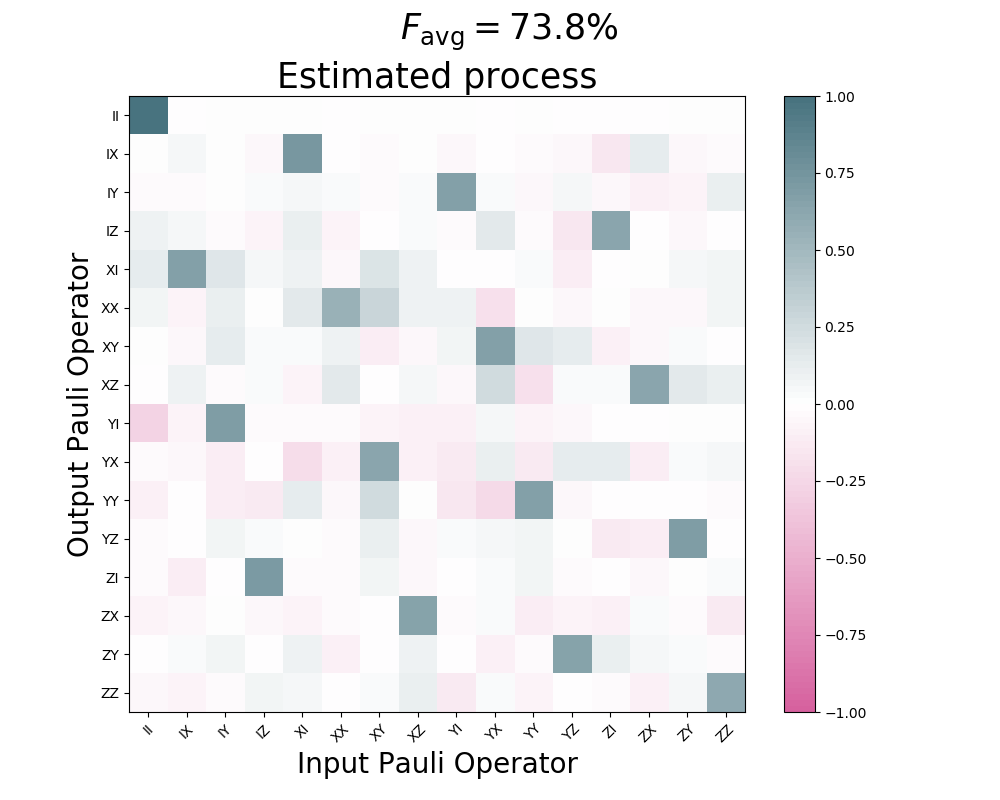
\includegraphics[width=1\linewidth]{process_tomography_qpu_8_13_SWAP_500} \caption{\label{fig:process_tomography_qpu_8_13_SWAP_500}}
\end{subfigure}
\begin{subfigure}[b]{0.5\textwidth}
   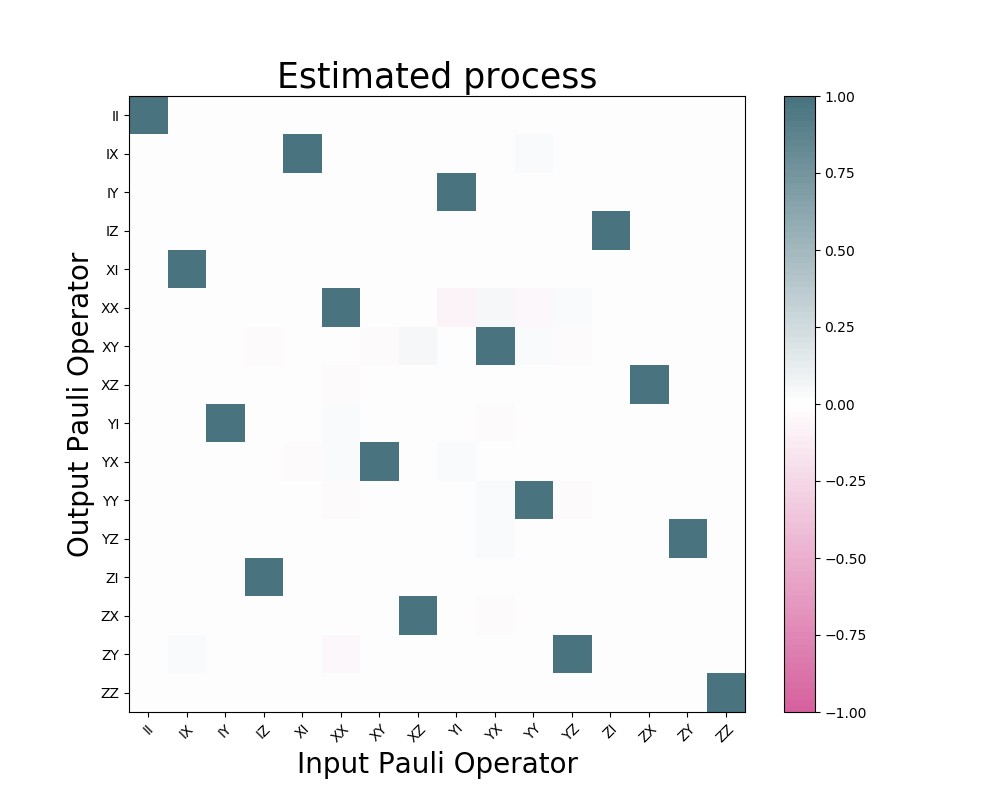
\includegraphics[width=1\linewidth]{process_tomography_qvm8_13_SWAP_2000}
\caption{\label{fig:process_tomography_qvm8_13_SWAP_2000}}
\end{subfigure}
\caption[]{The Pauli transfer matrix $\mathcal{R}_{ij}$ representation of the QPT completed for the SWAP gate run on the (a) QPU providing and (b) QVM which models the result for a errorless SWAP gate implementation.}
\end{figure}

Visualisation and information about $\mathcal{E}$ for QPT of the SWAP gate is represented by $\mathcal{R}$ in Fig. (\ref{fig:process_tomography_qpu_8_13_SWAP_500}) where the real coefficients are within [-1,1]. The SWAP gate provides an interesting result due to $F_{G}$ being considerably smaller in comparison to the other two-qubit gates. However, this is not surprising considering the SWAP gate is implemented by a circuit consisting of Hadamard and CZ gates. The noisy QVM continually timed out and could not compute QPT for the SWAP gate. The Pauli transfer matrix enables the comparison between $\mathcal{E}_{SWAP}$ and the approximately perfect $U_{SWAP}$ gate. QPT of the QVM without the noise model applied provides $U_{SWAP}$. However, as shown in Fig. (\ref{fig:process_tomography_qvm8_13_SWAP_2000}) there is still the presence of some small errors in $U_{SWAP}$.

Properties of $\mathcal{E}$ can be extracted from $\mathcal{R}$. Firstly, for $\mathcal{E}$ to be trace-preserving $Tr(P_{j})=Tr(\mathcal{E} (P_{j}))=\delta_{0j}$. Therefore applying these conditions to Eq.(\ref{eq:PTM}) results in $\mathcal{R}_{0j}=\delta_{0j}$. Similarly, the condition for unitality, $\mathcal{E} (I) = I$, requires $\mathcal{R}_{i0} = \delta_{0i}$. It is more complicated to determine if $\mathcal{E}$ is completely positive as this requires representation in the Choi matrix to be positive-semidefinite $^{[}$\citep{Chow2012UniversalQubits}$^{]}$. Therefore despite the representation of $U_{SWAP}$ in Fig. (\ref{fig:process_tomography_qpu_8_13_SWAP_500}) being unital and trace-preserving, $\mathcal{E}_{SWAP}$ is only trace-preserving due to the significant average gate error. The QPT function also enables the $\chi$ and Choi-matrix to be extracted. The real elements of the $\chi$-matrix of the $U_{SWAP}$ are shown in Fig.(\ref{fig:qvmSWAP}).

\begin{figure}[t]
\centering
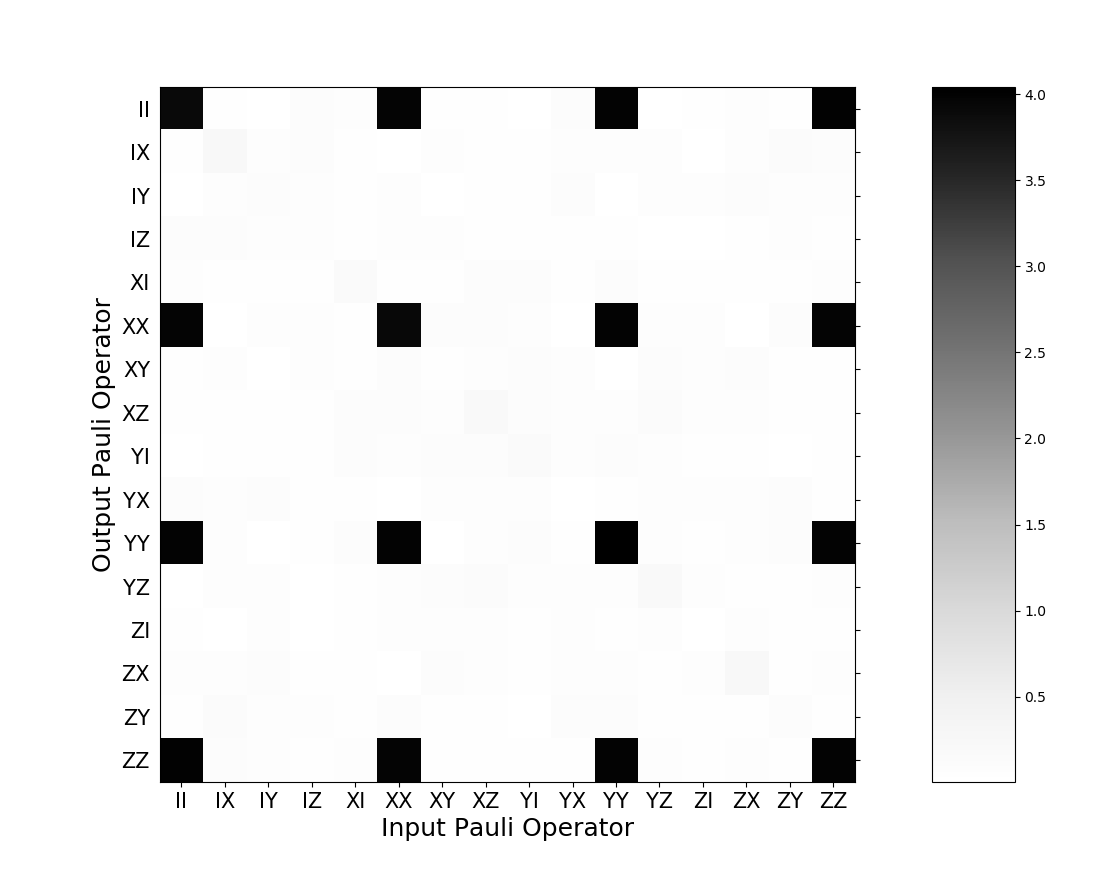
\includegraphics[height=0.35\textwidth,keepaspectratio]{qvmSWAP}
\caption{\label{fig:qvmSWAP} The process matrix $\chi$ representation of QPT completed for the SWAP gate run on the QVM $^{[}$\citep{Chow2012UniversalQubits}$^{]}$.}
\end{figure}


\subsection{Random Circuit QPT}
The random circuit generator game is set up such that the user selects the number of qubits and circuit depth to decide the difficultly level. To win the game the user must sufficiently reproduce the probability distribution of the output states. Therefore, to enable this game to run on the QPU it is useful to measure the average gate fidelity of a random selection of gates.

To estimate the error threshold, as shown in Table. \ref{tab:table2} QPT is completed for random sequences of single qubit gates. For each circuit depth QPT of the random circuit generated is repeated five times and the lowest $F_{G}$ obtained is presented. However, for two-qubit gates from Table \ref{tab:table1} it is clear that $F_{G}$ for the SWAP gate generates the greatest error rate. Therefore to estimate the two-qubit error threshold for each circuit depth an additional SWAP gate is applied and QPT is repeated twice.

\begin{table}[h!]
  \begin{center}
    \caption{Minimum $F_{G}$ for single qubit random gate sequence and increasing numbers of two-qubit SWAP gates.}
    \label{tab:table2}
    \begin{tabular}{l|r|r|l|r|r} % <-- Changed to S here.
      Circuit & single qubit & two-qubit \\
      depth & $F_{G}$ & $F_{G}$ \\
       \hline
      1 & 0.969 & 0.738 \\
      2 & 0.965 & 0.729 \\
      3 & 1.00 & 0.070 \\          
    \end{tabular}
  \end{center}
\end{table}


  
\subsection{Ramdomised Benchmarking}

Randomised benchmarking of a single qubit was completed by applying $V$ to the $\ket{0}$ input state of qubit 8 followed by applying $V^{\dagger}$ to return the inital state in the case of no errors. A random sequence of $R_{z}(\pi)$ and $R_{x}(\pi)$ form $V$ where the number of gates in the sequence increased up to 390. Each sequence step is repeated 500 times to gain the average sequence fidelity. Randomised benchmarking is insensitive to state preparation and measurement errors as these errors can be absorbed by constants when applying the fit model presented in Ref. [\citen{Magesan2011ScalableProcesses}]. For the simplest estimation, the average gate fidelity is taken as 0.999 from the exponential fit applied in Fig.(\ref{fig:randomisedbenchmarking}). The exponential nature of the decay in fidelity is observed more clearly in Ref. (\citen{Proctor2017WhatMeasures}) where the sequence of Clifford gates is extended to 2000 gates.   

\begin{figure}[t]
\centering
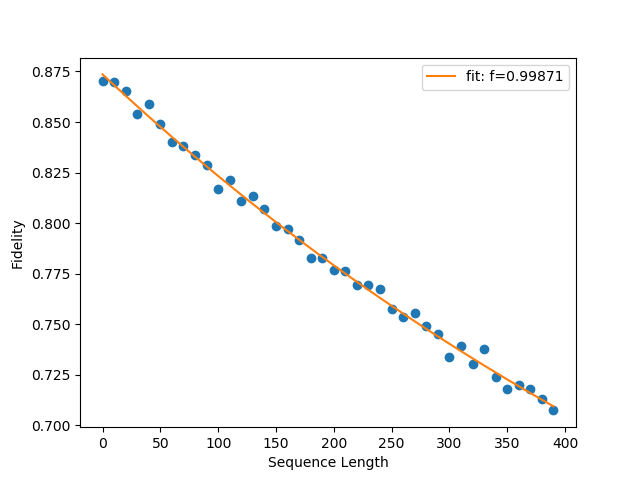
\includegraphics[height=0.35\textwidth,keepaspectratio]{randomisedbenchmarking}
\caption{\label{fig:randomisedbenchmarking}Average sequence fidelity vs. the random gate sequence length} 
\end{figure}


%exponential fit https://arxiv.org/pdf/1702.01853.pdf

 
